\documentclass[11pt, twocolumn]{article}

\usepackage{cite}
\usepackage{graphicx}
\usepackage[english]{babel}
\usepackage{authblk}
\usepackage[T1]{fontenc}
\usepackage[utf8]{inputenc}
\usepackage{indentfirst}
\usepackage{titlesec}
\usepackage{blindtext}
\DeclareGraphicsExtensions{.png}

\titlespacing\section{0pt}{12pt plus 4pt minus 2pt}{5pt plus 2pt minus 2pt}
\titleformat{\section}
{\normalfont\large\bfseries}{\thesection}{1em}{}

\title{Hybrid Applications: The End of Native Development?}
\author[1]{Andrew Zurn\\Computer Science Department\\Saint John's University\\Collegeville, MN\\awzurn@csbsju.edu}

\begin{document}
\maketitle
\begin{abstract}
Developing mobile applications has become one of the major topics within the technology industry, as the use of traditional desktops have begun to be replaced by mobile devices.  With the ever increasing need to develop mobile apps for the large range of varying operating systems and frameworks, developers have begun to adopt a new paradigm for creating applications.  'Hybrid' applications, a relatively new framework has emerged that leverages a common code base using web technologies to build applications for many of the popular mobile platforms, such as for iOS and Android.  Over the next few years, this new way of writing one application that will deploy across the spectrum of mobile devices, as it continues to grow and become a known alternative, will replace solely native development for building mobile applications.
\end{abstract}

\section{Introduction}
Mobile application development is rapidly becoming a necessity for anyone planning on building applications targeted at the main consumer markets, as today many people are shifting away from the traditional desktop to tablets, smart-phones, and other mobile devices.  Not only are people having to worry about adopting a mobile solution for their applications, they are also having to factor in the wide variety of devices and large range of operating systems and frameworks on these devices.  Native application development, that is developing with a platform's specific language (such as Objective-C for iOS and Java/XML for Android), has been almost the sole approach to developing the powerful, feature-rich apps that users have come to expect.  However, as Michael Nebeling in his paper, "Informing the Design of New Mobile Development Methods and Tools," states "given the diversity of device characteristics," native development poses a "major challenge" in creating, testing, and maintaining the various applications targeted at the current market of mobile technology, and only makes the mobile development process more difficult and time consuming. ~\cite{Nebeling2013}\\

Due to the fact of this proliferation of mobile operating systems and the evolution of the development platforms, a new option has recently been introduced, known as hybrid application development, which offers a solution to the problems that developing native applications has created.  Luis Corral, in his article, "Evolution of Mobile Software Development from Platform-Specific to Web-Based Multiplatform Paradigm," observes that this new approach will

\begin{quote}
change the way mobile applications are developed, as this approach slims down the mobile software development process and broads it impact.  It opens the opportunity of reducing development costs and relieves the problems associated with target-specific development, such as translating from language to language, using different platforms or dealing with redundant efforts of coding, testing and deployment. Finally, it will allow developers to structure a software process for a variety of platforms, targeting their final products to a wider extent of potential customers by conducting a single development process only. ~\cite{Corral2011}
\end{quote}

In short, as Corral exclaims and as will be further developed through this paper, this new "hybrid" technology does have the potential to redefine the status quo in mobile development and will, as developers abandon old native frameworks and replace it with these web-centric development environments.\\

\section{Hybrid Development}
Hybrid application development, although relatively new in the mobile spectrum, actually is based on mostly web technologies.  Corral briefly examines a few hybrid solutions, such as {\it PhoneGap}, and {\it Appcelerator}, which "both provide the means to develop applications with a technology-neutral point of view based on JavaScript, HTML, and CSS, allowing a single development to be deployed on diverse target platforms." ~\cite{Corral2011}  In addition to this common base of code using web technologies, the platforms also use each devices software development kit (SDK) to built the native components (buttons, text, devices features, etc.) and connects the HTML/CSS/JavaScript to it in order to add the dynamic operations of the application. ~\cite{Heitkoetter2013}  There are various different ways that this hybrid  approach achieves deployment to the large variety of platforms, such as using tools like {\it PhoneGap} or {\it Appcelerator}, among many other tools and frameworks. ~\cite{Goaer2013}

\section{The Future of Mobile Development}
Mobile application development has seen its shift in popularity and technologies used since its introduction in 2008. Having gone from developing with solely HTML and CSS, to platform dependent SDKs, now it is seeing another shift towards hybrid platforms that leverage both native and web development frameworks.  The next few years will likely see a renewed shift away from developing with native SKDs, as the solution that hybrid development poses becomes more refined, and the apps that it produces become more and more like their native counterparts.\\

\begin{figure*}[ht]
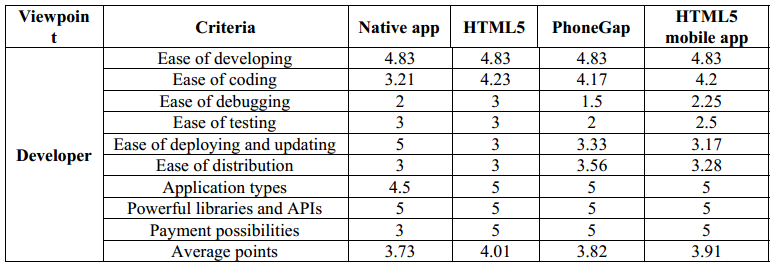
\includegraphics[width=\textwidth, height=3.5cm]{hybrid-native-compare-table}
\caption{Comparison of Native, HTML5, and Hybrid Development ~\cite{Huy2012}}
\end{figure*}

There are various reasons as to why developing native applications will begin to be replaced by developing with hybrid solutions.  One of the first is simply how large and unsustainable developing native apps has already become.  As Olivier Goaer points out in his article, "Yet Another DSL for Cross-Platform Mobile Development," with every major platform coming out with their own SDKs that are vastly different development tools and languages, this has lead to a "lack of sustainability" in the current development paradigm.  He goes onto say that platforms that fulfill the common programming slogan, "write once, run everywhere" will return "centre-stage," and these hybrid platform that allow developers to build one application and port it to many devices will replace the current native-driven trend. ~\cite{Goaer2013}\\

Another reason that hybrid development will replace natively developed applications is that hybrid applications are overall a lot easier to code and maintain.  Ngu Phuc Huy and Do vanThanh, in their article "Evaluation of mobile app paradigms," offer a quantified comparison of developing a native application compared to a hybrid application.  As can be seen in Figure 1, not only coding their hybrid application using {\it PhoneGap} was easier than developing their native application, the overall experience of using {\it PhoneGap} to develop in was better than developing natively. ~\cite{Huy2012}\\

As many of the hybrid technologies use JavaScript as their core means of adding the dynamic features that are central to mobile applications, this means the performance of the JavaScript engine is another main factor in hybrid development adoption.  Brian Leroux and Andre Charland, in their article, "Mobile Application Development: Web vs. Native," examine this point, and state that when "pitting JavaScript against compiled languages... JavaScript is holding its own." They also go onto say that "this isn't surprising - JavaScript virtual machine technology is the new front line for the browser wars... The bottom line is that heavy spending by al the major players is fueling this JavaScript arms race," which in turn is only helping the development process and power that these hybrid solutions offer.  In short, as JavaScript becomes more powerful, a lot of the hybrid development environments and also the applications that they build become more powerful as well. ~\cite{Leroux2011} \\

The hybrid platforms also offer a better solution than native development due to the commonness and generality of the knowledge and skills that they use. Due to the fact that so many developers either know or have had some experiences with the HTML/CSS/JavaScript web stack, developing these applications will not need the skills and expertise that their native counterparts require.  In an {\it Appcelerator} white paper, they highlight this fact as they state,

\begin{quote}
It's widely believed that there are far more HTML and JavaScript than Objective-C developers.  Enterprises have spent the last 15 years building up internal developer expertise in web technologies... In a recent study, JavaScript and HTML5 held 2 of the top 4 rankings of 18 different programming and markup language frameworks. ~\cite{Appcelerator.com2012}
\end{quote}

Not only will the web programming languages offer more universal access and also a support base for those developing hybrid applications, but it will also allow for a large increase in code re-usability. {\it Appcelerator} also solidifies this, as they proclaim that when using a hybrid solution,\\

\begin{quote}
A single team with JavaScript experience can build an app for iOS, Android, BlackBerry, and HTML5, with up to 90\% code reuse.  The result is significantly lower cost and faster time to market. ~\cite{Appcelerator.com2012}
\end{quote}

As the same resources are used to build the multiple native applications, large sections of code and other application resources will be utilized, and thus will produce less work, increase time use, and improve the overall maintainability of the code.

Overall, the reasons as to why hybrid application development will eventually take over the mobile development spectrum can be summed up in the visual proved by Shahar Kaminitz, the CEO of WorkLight.com. As can be seen, and as has been discussed, hybrid apps are starting to hold their own against native apps. When looking at this figure, we see that the only drawback it has when compared against a native application is performance, but even this is becoming less noticeable as there is currently an effort to bridge that gap.  In the end, as Brian Leroux states, although hybrid development has not achieved" native performance just yet, "it is getting close." ~\cite{Leroux2011}.

\begin{figure}[h]
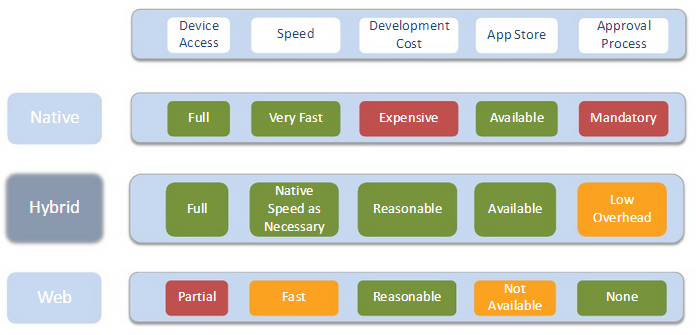
\includegraphics[scale=0.5]{ComparativeTable}
\caption{Comparative Table between Different Development Approaches} ~\cite{Kaminitz2012}
\end{figure}

\section{Conclusion}
Developing natively has been the major trend in creating mobile apps since the major introduction of the smart-phone.  The obvious reason for this is that there was a wide array of powerful tools it gave developers that accessed many of a devices rich features.  These tools were also greatly supported and new and exciting features were always being added, and it was also one, if not the only way to install applications right onto a device.  Now, however, this has changed, as many tools are being rapidly developed and supported to build applications that attain the goal of cross-platform compatibility.  Hybrid applications development is becoming a major contender in the mobile app development arena, and as it grows closer in achieving the performance, look and feel of native applications, it will one day replace how mobile apps have been mainly developed.  However, as Huy and Leroux point out, that day is not quite here, but soon will be. ~\cite{Huy2012} ~\cite{Leroux2011}\\

These hybrid development environments, outside of beginning to perform just as well as their native counterparts, will also renew and bring about a more sustainable coding paradigm. ~\cite{Goaer2013}  "Conducting the whole development process for a single application for each platform will eventually become redundant, expensive and unpractical," states Luis Corral. ~\cite{Corral2011}  With the rapid growth of our new solution, no longer will developers need to build applications specifically for each platform, but rather they will be able to build a single application out of a common base of technologies that are widely used across the development landscape, and will also able to reach almost 90\% of the mobile market (with app developed for just Android and iOS). ~\cite{Llamas2013}

Over the next five years, hybrid developed applications will become the new standard for creating mobile applications. Luis Corral boldly exclaims that as these hybrid development environments "evolve to offer an integral native development solution," mobile application developers will come to replace the status quo with these tools thanks to "their versatility, economy and usefulness, lesser dependence on platforms and SDKs, and full functionality and reliability in comparison to their binary counterparts." ~\cite{Corral2011}  Hybrid applications will ultimately become the new way to develop native applications, and the differences between how they look, feel and act, will soon be indistinguishable.\\


\bibliographystyle{plain}
\bibliography{FutureTrendsBibs}
\end{document}